% begin module definite-integral-negative
\begin{frame}
\begin{columns}
\column{.55\textwidth}
\begin{itemize}
\item  We know already that if $f(x)$ is always positive, then $\int_a^bf(x)\diff x$ is the area under the curve.
\end{itemize}
\column{.45\textwidth}
\psset{xunit=2cm, yunit=2cm}
\begin{pspicture}(-5, -5)(5,5) 
\psline{linecolor=red!1}(0, -0.3)(0, -0.31)
\psframe*[linecolor=white](-5,-5)(5,5) 
\psaxes[ticks=none, labels=none]{<->}(0,0)(-0.1,-0.1)(1.4,1.4)
\tiny
\psline(-0.05, 1)(0.05,1)
\rput[r] (-0.07,1){$1$}
%Function formula: x^{2} 
\rput(0.9,1.3){$y=x^{2}$} 
\uncover<1>{
%approximation 1/3
\psline*[linecolor=\psColorAreaUnderGraph, linewidth=0.1pt](0.333333, 0)(0.333333, 0.111111)(0, 0.111111)(0, 0)(0.666667, 0)(0.666667, 0.444444)(0.333333, 0.444444)(0.333333, 0)(1, 0)(1, 1)(0.666667, 1)(0.666667, 0)
\psline[linecolor=blue, linewidth=0.1pt](0.333333, 0)(0.333333, 0.111111)(0, 0.111111)(0, 0)(0.666667, 0)(0.666667, 0.444444)(0.333333, 0.444444)(0.333333, 0)(1, 0)(1, 1)(0.666667, 1)(0.666667, 0)
\rput[t](0.333333,-0.03){$\frac{1}{3}$}\rput[t](0.666667,-0.03){$\frac{2}{3}$}\rput[t](1,-0.03){$1$}
}
\uncover<2>{
%approximation 1/4
\psline*[linecolor=\psColorAreaUnderGraph, linewidth=0.1pt](0.25, 0)(0.25, 0.0625)(0, 0.0625)(0, 0)(0.5, 0)(0.5, 0.25)(0.25, 0.25)(0.25, 0)(0.75, 0)(0.75, 0.5625)(0.5, 0.5625)(0.5, 0)(1, 0)(1, 1)(0.75, 1)(0.75, 0)
\psline[linecolor=blue, linewidth=0.1pt](0.25, 0)(0.25, 0.0625)(0, 0.0625)(0, 0)(0.5, 0)(0.5, 0.25)(0.25, 0.25)(0.25, 0)(0.75, 0)(0.75, 0.5625)(0.5, 0.5625)(0.5, 0)(1, 0)(1, 1)(0.75, 1)(0.75, 0)
\rput[t](0.25,-0.03){$\frac{1}{4}$}\rput[t](0.5,-0.03){$\frac{1}{2}$}\rput[t](0.75,-0.03){$\frac{3}{4}$}\rput[t](1,-0.03){$1$}
}
\uncover<3>{
%approximation 1/5
\psline*[linecolor=\psColorAreaUnderGraph, linewidth=0.1pt](0.2, 0)(0.2, 0.04)(0, 0.04)(0, 0)(0.4, 0)(0.4, 0.16)(0.2, 0.16)(0.2, 0)(0.6, 0)(0.6, 0.36)(0.4, 0.36)(0.4, 0)(0.8, 0)(0.8, 0.64)(0.6, 0.64)(0.6, 0)(1, 0)(1, 1)(0.8, 1)(0.8, 0)
\psline[linecolor=blue, linewidth=0.1pt](0.2, 0)(0.2, 0.04)(0, 0.04)(0, 0)(0.4, 0)(0.4, 0.16)(0.2, 0.16)(0.2, 0)(0.6, 0)(0.6, 0.36)(0.4, 0.36)(0.4, 0)(0.8, 0)(0.8, 0.64)(0.6, 0.64)(0.6, 0)(1, 0)(1, 1)(0.8, 1)(0.8, 0)
\rput[t](0.2,-0.03){$\frac{1}{5}$}\rput[t](0.4,-0.03){$\frac{2}{5}$}\rput[t](0.6,-0.03){$\frac{3}{5}$}\rput[t](0.8,-0.03){$\frac{4}{5}$}\rput[t](1,-0.03){$1$}
}
\uncover<4>{
%approximation 1/8
\psline*[linecolor=\psColorAreaUnderGraph, linewidth=0.1pt](0.125, 0)(0.125, 0.015625)(0, 0.015625)(0, 0)(0.25, 0)(0.25, 0.0625)(0.125, 0.0625)(0.125, 0)(0.375, 0)(0.375, 0.140625)(0.25, 0.140625)(0.25, 0)(0.5, 0)(0.5, 0.25)(0.375, 0.25)(0.375, 0)(0.625, 0)(0.625, 0.390625)(0.5, 0.390625)(0.5, 0)(0.75, 0)(0.75, 0.5625)(0.625, 0.5625)(0.625, 0)(0.875, 0)(0.875, 0.765625)(0.75, 0.765625)(0.75, 0)(1, 0)(1, 1)(0.875, 1)(0.875, 0)
\psline[linecolor=blue, linewidth=0.1pt](0.125, 0)(0.125, 0.015625)(0, 0.015625)(0, 0)(0.25, 0)(0.25, 0.0625)(0.125, 0.0625)(0.125, 0)(0.375, 0)(0.375, 0.140625)(0.25, 0.140625)(0.25, 0)(0.5, 0)(0.5, 0.25)(0.375, 0.25)(0.375, 0)(0.625, 0)(0.625, 0.390625)(0.5, 0.390625)(0.5, 0)(0.75, 0)(0.75, 0.5625)(0.625, 0.5625)(0.625, 0)(0.875, 0)(0.875, 0.765625)(0.75, 0.765625)(0.75, 0)(1, 0)(1, 1)(0.875, 1)(0.875, 0)
\rput[t](0.125,-0.03){$\frac{1}{8}$}\rput[t](0.25,-0.03){$\frac{1}{4}$}\rput[t](0.375,-0.03){$\frac{3}{8}$}\rput[t](0.5,-0.03){$\frac{1}{2}$}\rput[t](0.625,-0.03){$\frac{5}{8}$}\rput[t](0.75,-0.03){$\frac{3}{4}$}\rput[t](0.875,-0.03){$\frac{7}{8}$}\rput[t](1,-0.03){$1$}
}
\uncover<5>{
%approximation 1/10
\psline*[linecolor=\psColorAreaUnderGraph, linewidth=0.1pt](0.1, 0)(0.1, 0.01)(0, 0.01)(0, 0)(0.2, 0)(0.2, 0.04)(0.1, 0.04)(0.1, 0)(0.3, 0)(0.3, 0.09)(0.2, 0.09)(0.2, 0)(0.4, 0)(0.4, 0.16)(0.3, 0.16)(0.3, 0)(0.5, 0)(0.5, 0.25)(0.4, 0.25)(0.4, 0)(0.6, 0)(0.6, 0.36)(0.5, 0.36)(0.5, 0)(0.7, 0)(0.7, 0.49)(0.6, 0.49)(0.6, 0)(0.8, 0)(0.8, 0.64)(0.7, 0.64)(0.7, 0)(0.9, 0)(0.9, 0.81)(0.8, 0.81)(0.8, 0)(1, 0)(1, 1)(0.9, 1)(0.9, 0)
\psline[linecolor=blue, linewidth=0.1pt](0.1, 0)(0.1, 0.01)(0, 0.01)(0, 0)(0.2, 0)(0.2, 0.04)(0.1, 0.04)(0.1, 0)(0.3, 0)(0.3, 0.09)(0.2, 0.09)(0.2, 0)(0.4, 0)(0.4, 0.16)(0.3, 0.16)(0.3, 0)(0.5, 0)(0.5, 0.25)(0.4, 0.25)(0.4, 0)(0.6, 0)(0.6, 0.36)(0.5, 0.36)(0.5, 0)(0.7, 0)(0.7, 0.49)(0.6, 0.49)(0.6, 0)(0.8, 0)(0.8, 0.64)(0.7, 0.64)(0.7, 0)(0.9, 0)(0.9, 0.81)(0.8, 0.81)(0.8, 0)(1, 0)(1, 1)(0.9, 1)(0.9, 0)
\rput[t](0.1,-0.03){$\frac{1}{10}$}\rput[t](0.2,-0.03){$\frac{1}{5}$}\rput[t](0.3,-0.03){$\frac{3}{10}$}\rput[t](0.4,-0.03){$\frac{2}{5}$}\rput[t](0.5,-0.03){$\frac{1}{2}$}\rput[t](0.6,-0.03){$\frac{3}{5}$}\rput[t](0.7,-0.03){$\frac{7}{10}$}\rput[t](0.8,-0.03){$\frac{4}{5}$}\rput[t](0.9,-0.03){$\frac{9}{10}$}\rput[t](1,-0.03){$1$}
}
\uncover<6>{
%approximation 1/20
\psline*[linecolor=\psColorAreaUnderGraph, linewidth=0.1pt](0.05, 0)(0.05, 0.0025)(0, 0.0025)(0, 0)(0.1, 0)(0.1, 0.01)(0.05, 0.01)(0.05, 0)(0.15, 0)(0.15, 0.0225)(0.1, 0.0225)(0.1, 0)(0.2, 0)(0.2, 0.04)(0.15, 0.04)(0.15, 0)(0.25, 0)(0.25, 0.0625)(0.2, 0.0625)(0.2, 0)(0.3, 0)(0.3, 0.09)(0.25, 0.09)(0.25, 0)(0.35, 0)(0.35, 0.1225)(0.3, 0.1225)(0.3, 0)(0.4, 0)(0.4, 0.16)(0.35, 0.16)(0.35, 0)(0.45, 0)(0.45, 0.2025)(0.4, 0.2025)(0.4, 0)(0.5, 0)(0.5, 0.25)(0.45, 0.25)(0.45, 0)(0.55, 0)(0.55, 0.3025)(0.5, 0.3025)(0.5, 0)(0.6, 0)(0.6, 0.36)(0.55, 0.36)(0.55, 0)(0.65, 0)(0.65, 0.4225)(0.6, 0.4225)(0.6, 0)(0.7, 0)(0.7, 0.49)(0.65, 0.49)(0.65, 0)(0.75, 0)(0.75, 0.5625)(0.7, 0.5625)(0.7, 0)(0.8, 0)(0.8, 0.64)(0.75, 0.64)(0.75, 0)(0.85, 0)(0.85, 0.7225)(0.8, 0.7225)(0.8, 0)(0.9, 0)(0.9, 0.81)(0.85, 0.81)(0.85, 0)(0.95, 0)(0.95, 0.9025)(0.9, 0.9025)(0.9, 0)(1, 0)(1, 1)(0.95, 1)(0.95, 0)
\psline[linecolor=blue, linewidth=0.1pt](0.05, 0)(0.05, 0.0025)(0, 0.0025)(0, 0)(0.1, 0)(0.1, 0.01)(0.05, 0.01)(0.05, 0)(0.15, 0)(0.15, 0.0225)(0.1, 0.0225)(0.1, 0)(0.2, 0)(0.2, 0.04)(0.15, 0.04)(0.15, 0)(0.25, 0)(0.25, 0.0625)(0.2, 0.0625)(0.2, 0)(0.3, 0)(0.3, 0.09)(0.25, 0.09)(0.25, 0)(0.35, 0)(0.35, 0.1225)(0.3, 0.1225)(0.3, 0)(0.4, 0)(0.4, 0.16)(0.35, 0.16)(0.35, 0)(0.45, 0)(0.45, 0.2025)(0.4, 0.2025)(0.4, 0)(0.5, 0)(0.5, 0.25)(0.45, 0.25)(0.45, 0)(0.55, 0)(0.55, 0.3025)(0.5, 0.3025)(0.5, 0)(0.6, 0)(0.6, 0.36)(0.55, 0.36)(0.55, 0)(0.65, 0)(0.65, 0.4225)(0.6, 0.4225)(0.6, 0)(0.7, 0)(0.7, 0.49)(0.65, 0.49)(0.65, 0)(0.75, 0)(0.75, 0.5625)(0.7, 0.5625)(0.7, 0)(0.8, 0)(0.8, 0.64)(0.75, 0.64)(0.75, 0)(0.85, 0)(0.85, 0.7225)(0.8, 0.7225)(0.8, 0)(0.9, 0)(0.9, 0.81)(0.85, 0.81)(0.85, 0)(0.95, 0)(0.95, 0.9025)(0.9, 0.9025)(0.9, 0)(1, 0)(1, 1)(0.95, 1)(0.95, 0)
}
\uncover<7>{
%approximation 1/30
\psline*[linecolor=\psColorAreaUnderGraph, linewidth=0.1pt](0.0333333, 0)(0.0333333, 0.00111111)(0, 0.00111111)(0, 0)(0.0666667, 0)(0.0666667, 0.00444444)(0.0333333, 0.00444444)(0.0333333, 0)(0.1, 0)(0.1, 0.01)(0.0666667, 0.01)(0.0666667, 0)(0.133333, 0)(0.133333, 0.0177778)(0.1, 0.0177778)(0.1, 0)(0.166667, 0)(0.166667, 0.0277778)(0.133333, 0.0277778)(0.133333, 0)(0.2, 0)(0.2, 0.04)(0.166667, 0.04)(0.166667, 0)(0.233333, 0)(0.233333, 0.0544444)(0.2, 0.0544444)(0.2, 0)(0.266667, 0)(0.266667, 0.0711111)(0.233333, 0.0711111)(0.233333, 0)(0.3, 0)(0.3, 0.09)(0.266667, 0.09)(0.266667, 0)(0.333333, 0)(0.333333, 0.111111)(0.3, 0.111111)(0.3, 0)(0.366667, 0)(0.366667, 0.134444)(0.333333, 0.134444)(0.333333, 0)(0.4, 0)(0.4, 0.16)(0.366667, 0.16)(0.366667, 0)(0.433333, 0)(0.433333, 0.187778)(0.4, 0.187778)(0.4, 0)(0.466667, 0)(0.466667, 0.217778)(0.433333, 0.217778)(0.433333, 0)(0.5, 0)(0.5, 0.25)(0.466667, 0.25)(0.466667, 0)(0.533333, 0)(0.533333, 0.284444)(0.5, 0.284444)(0.5, 0)(0.566667, 0)(0.566667, 0.321111)(0.533333, 0.321111)(0.533333, 0)(0.6, 0)(0.6, 0.36)(0.566667, 0.36)(0.566667, 0)(0.633333, 0)(0.633333, 0.401111)(0.6, 0.401111)(0.6, 0)(0.666667, 0)(0.666667, 0.444444)(0.633333, 0.444444)(0.633333, 0)(0.7, 0)(0.7, 0.49)(0.666667, 0.49)(0.666667, 0)(0.733333, 0)(0.733333, 0.537778)(0.7, 0.537778)(0.7, 0)(0.766667, 0)(0.766667, 0.587778)(0.733333, 0.587778)(0.733333, 0)(0.8, 0)(0.8, 0.64)(0.766667, 0.64)(0.766667, 0)(0.833333, 0)(0.833333, 0.694444)(0.8, 0.694444)(0.8, 0)(0.866667, 0)(0.866667, 0.751111)(0.833333, 0.751111)(0.833333, 0)(0.9, 0)(0.9, 0.81)(0.866667, 0.81)(0.866667, 0)(0.933333, 0)(0.933333, 0.871111)(0.9, 0.871111)(0.9, 0)(0.966667, 0)(0.966667, 0.934444)(0.933333, 0.934444)(0.933333, 0)(1, 0)(1, 1)(0.966667, 1)(0.966667, 0)
\psline[linecolor=blue, linewidth=0.1pt](0.0333333, 0)(0.0333333, 0.00111111)(0, 0.00111111)(0, 0)(0.0666667, 0)(0.0666667, 0.00444444)(0.0333333, 0.00444444)(0.0333333, 0)(0.1, 0)(0.1, 0.01)(0.0666667, 0.01)(0.0666667, 0)(0.133333, 0)(0.133333, 0.0177778)(0.1, 0.0177778)(0.1, 0)(0.166667, 0)(0.166667, 0.0277778)(0.133333, 0.0277778)(0.133333, 0)(0.2, 0)(0.2, 0.04)(0.166667, 0.04)(0.166667, 0)(0.233333, 0)(0.233333, 0.0544444)(0.2, 0.0544444)(0.2, 0)(0.266667, 0)(0.266667, 0.0711111)(0.233333, 0.0711111)(0.233333, 0)(0.3, 0)(0.3, 0.09)(0.266667, 0.09)(0.266667, 0)(0.333333, 0)(0.333333, 0.111111)(0.3, 0.111111)(0.3, 0)(0.366667, 0)(0.366667, 0.134444)(0.333333, 0.134444)(0.333333, 0)(0.4, 0)(0.4, 0.16)(0.366667, 0.16)(0.366667, 0)(0.433333, 0)(0.433333, 0.187778)(0.4, 0.187778)(0.4, 0)(0.466667, 0)(0.466667, 0.217778)(0.433333, 0.217778)(0.433333, 0)(0.5, 0)(0.5, 0.25)(0.466667, 0.25)(0.466667, 0)(0.533333, 0)(0.533333, 0.284444)(0.5, 0.284444)(0.5, 0)(0.566667, 0)(0.566667, 0.321111)(0.533333, 0.321111)(0.533333, 0)(0.6, 0)(0.6, 0.36)(0.566667, 0.36)(0.566667, 0)(0.633333, 0)(0.633333, 0.401111)(0.6, 0.401111)(0.6, 0)(0.666667, 0)(0.666667, 0.444444)(0.633333, 0.444444)(0.633333, 0)(0.7, 0)(0.7, 0.49)(0.666667, 0.49)(0.666667, 0)(0.733333, 0)(0.733333, 0.537778)(0.7, 0.537778)(0.7, 0)(0.766667, 0)(0.766667, 0.587778)(0.733333, 0.587778)(0.733333, 0)(0.8, 0)(0.8, 0.64)(0.766667, 0.64)(0.766667, 0)(0.833333, 0)(0.833333, 0.694444)(0.8, 0.694444)(0.8, 0)(0.866667, 0)(0.866667, 0.751111)(0.833333, 0.751111)(0.833333, 0)(0.9, 0)(0.9, 0.81)(0.866667, 0.81)(0.866667, 0)(0.933333, 0)(0.933333, 0.871111)(0.9, 0.871111)(0.9, 0)(0.966667, 0)(0.966667, 0.934444)(0.933333, 0.934444)(0.933333, 0)(1, 0)(1, 1)(0.966667, 1)(0.966667, 0)
}
\uncover<8>{
%approximation 1/40
\psline*[linecolor=\psColorAreaUnderGraph, linewidth=0.1pt](0.025, 0)(0.025, 0.000625)(0, 0.000625)(0, 0)(0.05, 0)(0.05, 0.0025)(0.025, 0.0025)(0.025, 0)(0.075, 0)(0.075, 0.005625)(0.05, 0.005625)(0.05, 0)(0.1, 0)(0.1, 0.01)(0.075, 0.01)(0.075, 0)(0.125, 0)(0.125, 0.015625)(0.1, 0.015625)(0.1, 0)(0.15, 0)(0.15, 0.0225)(0.125, 0.0225)(0.125, 0)(0.175, 0)(0.175, 0.030625)(0.15, 0.030625)(0.15, 0)(0.2, 0)(0.2, 0.04)(0.175, 0.04)(0.175, 0)(0.225, 0)(0.225, 0.050625)(0.2, 0.050625)(0.2, 0)(0.25, 0)(0.25, 0.0625)(0.225, 0.0625)(0.225, 0)(0.275, 0)(0.275, 0.075625)(0.25, 0.075625)(0.25, 0)(0.3, 0)(0.3, 0.09)(0.275, 0.09)(0.275, 0)(0.325, 0)(0.325, 0.105625)(0.3, 0.105625)(0.3, 0)(0.35, 0)(0.35, 0.1225)(0.325, 0.1225)(0.325, 0)(0.375, 0)(0.375, 0.140625)(0.35, 0.140625)(0.35, 0)(0.4, 0)(0.4, 0.16)(0.375, 0.16)(0.375, 0)(0.425, 0)(0.425, 0.180625)(0.4, 0.180625)(0.4, 0)(0.45, 0)(0.45, 0.2025)(0.425, 0.2025)(0.425, 0)(0.475, 0)(0.475, 0.225625)(0.45, 0.225625)(0.45, 0)(0.5, 0)(0.5, 0.25)(0.475, 0.25)(0.475, 0)(0.525, 0)(0.525, 0.275625)(0.5, 0.275625)(0.5, 0)(0.55, 0)(0.55, 0.3025)(0.525, 0.3025)(0.525, 0)(0.575, 0)(0.575, 0.330625)(0.55, 0.330625)(0.55, 0)(0.6, 0)(0.6, 0.36)(0.575, 0.36)(0.575, 0)(0.625, 0)(0.625, 0.390625)(0.6, 0.390625)(0.6, 0)(0.65, 0)(0.65, 0.4225)(0.625, 0.4225)(0.625, 0)(0.675, 0)(0.675, 0.455625)(0.65, 0.455625)(0.65, 0)(0.7, 0)(0.7, 0.49)(0.675, 0.49)(0.675, 0)(0.725, 0)(0.725, 0.525625)(0.7, 0.525625)(0.7, 0)(0.75, 0)(0.75, 0.5625)(0.725, 0.5625)(0.725, 0)(0.775, 0)(0.775, 0.600625)(0.75, 0.600625)(0.75, 0)(0.8, 0)(0.8, 0.64)(0.775, 0.64)(0.775, 0)(0.825, 0)(0.825, 0.680625)(0.8, 0.680625)(0.8, 0)(0.85, 0)(0.85, 0.7225)(0.825, 0.7225)(0.825, 0)(0.875, 0)(0.875, 0.765625)(0.85, 0.765625)(0.85, 0)(0.9, 0)(0.9, 0.81)(0.875, 0.81)(0.875, 0)(0.925, 0)(0.925, 0.855625)(0.9, 0.855625)(0.9, 0)(0.95, 0)(0.95, 0.9025)(0.925, 0.9025)(0.925, 0)(0.975, 0)(0.975, 0.950625)(0.95, 0.950625)(0.95, 0)(1, 0)(1, 1)(0.975, 1)(0.975, 0)
\psline[linecolor=blue, linewidth=0.1pt](0.025, 0)(0.025, 0.000625)(0, 0.000625)(0, 0)(0.05, 0)(0.05, 0.0025)(0.025, 0.0025)(0.025, 0)(0.075, 0)(0.075, 0.005625)(0.05, 0.005625)(0.05, 0)(0.1, 0)(0.1, 0.01)(0.075, 0.01)(0.075, 0)(0.125, 0)(0.125, 0.015625)(0.1, 0.015625)(0.1, 0)(0.15, 0)(0.15, 0.0225)(0.125, 0.0225)(0.125, 0)(0.175, 0)(0.175, 0.030625)(0.15, 0.030625)(0.15, 0)(0.2, 0)(0.2, 0.04)(0.175, 0.04)(0.175, 0)(0.225, 0)(0.225, 0.050625)(0.2, 0.050625)(0.2, 0)(0.25, 0)(0.25, 0.0625)(0.225, 0.0625)(0.225, 0)(0.275, 0)(0.275, 0.075625)(0.25, 0.075625)(0.25, 0)(0.3, 0)(0.3, 0.09)(0.275, 0.09)(0.275, 0)(0.325, 0)(0.325, 0.105625)(0.3, 0.105625)(0.3, 0)(0.35, 0)(0.35, 0.1225)(0.325, 0.1225)(0.325, 0)(0.375, 0)(0.375, 0.140625)(0.35, 0.140625)(0.35, 0)(0.4, 0)(0.4, 0.16)(0.375, 0.16)(0.375, 0)(0.425, 0)(0.425, 0.180625)(0.4, 0.180625)(0.4, 0)(0.45, 0)(0.45, 0.2025)(0.425, 0.2025)(0.425, 0)(0.475, 0)(0.475, 0.225625)(0.45, 0.225625)(0.45, 0)(0.5, 0)(0.5, 0.25)(0.475, 0.25)(0.475, 0)(0.525, 0)(0.525, 0.275625)(0.5, 0.275625)(0.5, 0)(0.55, 0)(0.55, 0.3025)(0.525, 0.3025)(0.525, 0)(0.575, 0)(0.575, 0.330625)(0.55, 0.330625)(0.55, 0)(0.6, 0)(0.6, 0.36)(0.575, 0.36)(0.575, 0)(0.625, 0)(0.625, 0.390625)(0.6, 0.390625)(0.6, 0)(0.65, 0)(0.65, 0.4225)(0.625, 0.4225)(0.625, 0)(0.675, 0)(0.675, 0.455625)(0.65, 0.455625)(0.65, 0)(0.7, 0)(0.7, 0.49)(0.675, 0.49)(0.675, 0)(0.725, 0)(0.725, 0.525625)(0.7, 0.525625)(0.7, 0)(0.75, 0)(0.75, 0.5625)(0.725, 0.5625)(0.725, 0)(0.775, 0)(0.775, 0.600625)(0.75, 0.600625)(0.75, 0)(0.8, 0)(0.8, 0.64)(0.775, 0.64)(0.775, 0)(0.825, 0)(0.825, 0.680625)(0.8, 0.680625)(0.8, 0)(0.85, 0)(0.85, 0.7225)(0.825, 0.7225)(0.825, 0)(0.875, 0)(0.875, 0.765625)(0.85, 0.765625)(0.85, 0)(0.9, 0)(0.9, 0.81)(0.875, 0.81)(0.875, 0)(0.925, 0)(0.925, 0.855625)(0.9, 0.855625)(0.9, 0)(0.95, 0)(0.95, 0.9025)(0.925, 0.9025)(0.925, 0)(0.975, 0)(0.975, 0.950625)(0.95, 0.950625)(0.95, 0)(1, 0)(1, 1)(0.975, 1)(0.975, 0)
}
\uncover<9->{
\pscustom*[linecolor=\psColorAreaUnderGraph, linewidth=0.1pt]{\psplot[linecolor=red, plotpoints=1000]{0}{1}{x 2 exp }\psline(1,1)(1,0)}
}
\psline(1,-0.03)(1,0.03)
\uncover<6->{
\rput[t] (1,-0.07){$1$}
}
\psplot[linecolor=red, plotpoints=1000]{0}{1.15}{x 2 exp }
\end{pspicture}
%\only<handout:0| -1>{%
%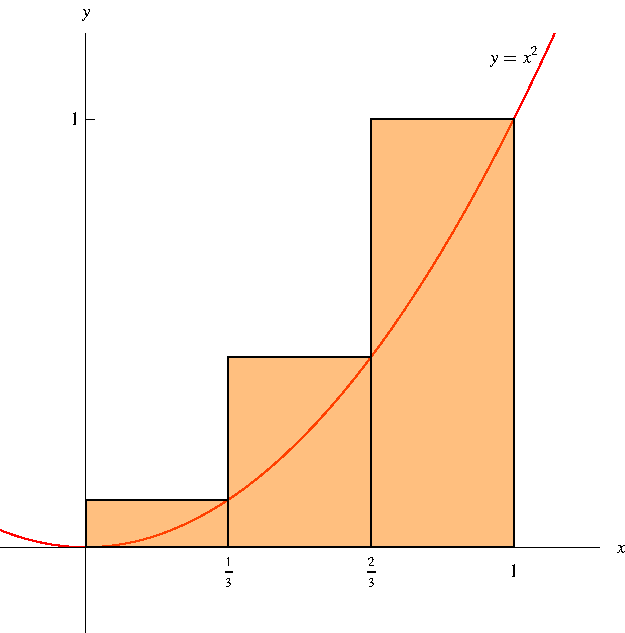
\includegraphics[height=4.2cm]{integration/pictures/05-01-righta.pdf}%
%}%
%\only<handout:0| 2>{%
%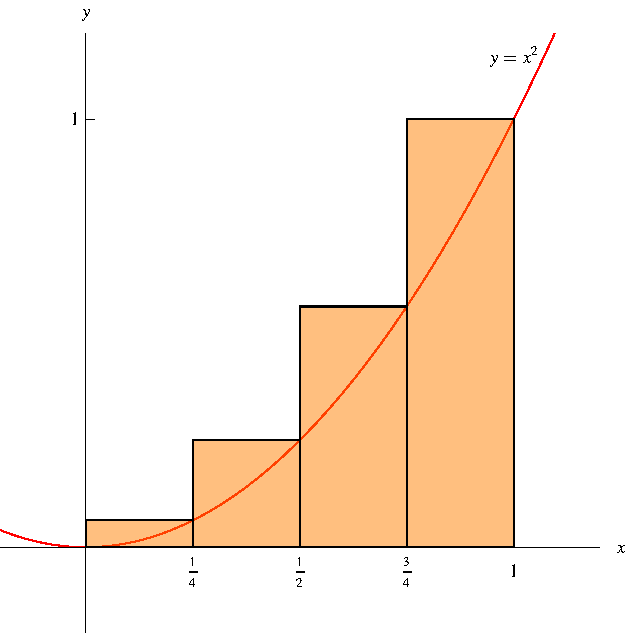
\includegraphics[height=4.2cm]{integration/pictures/05-01-rightb.pdf}%
%}%
%\only<handout:0| 3>{%
%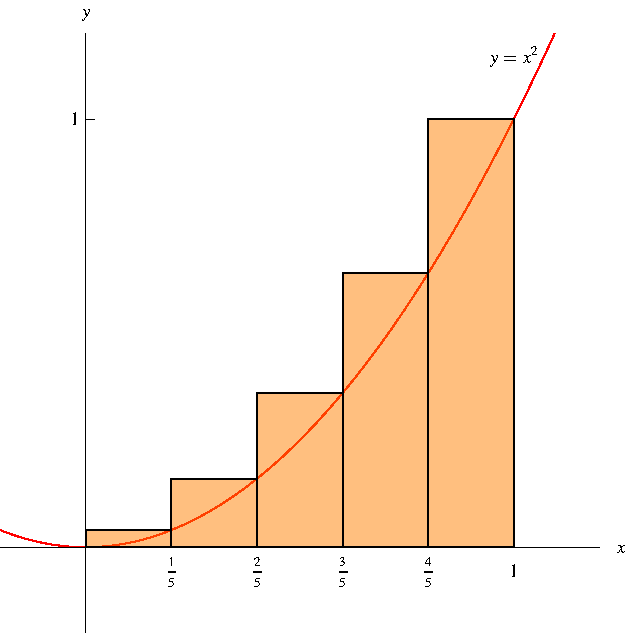
\includegraphics[height=4.2cm]{integration/pictures/05-01-rightc.pdf}%
%}%
%\only<handout:0| 4>{%
%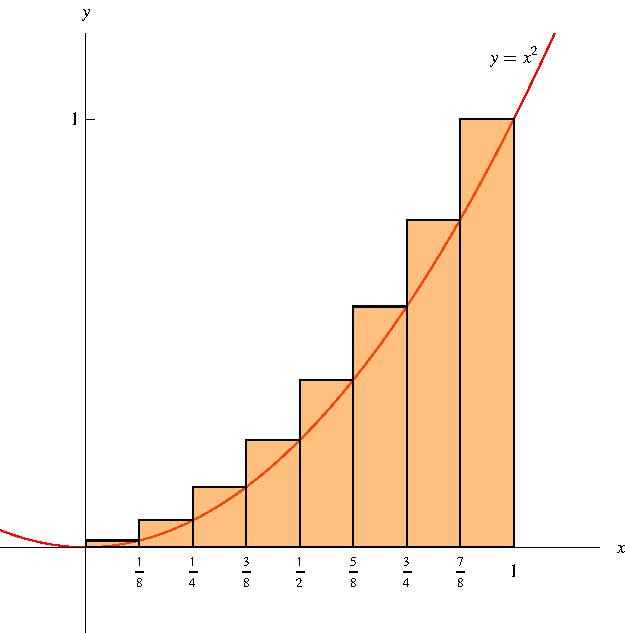
\includegraphics[height=4.2cm]{integration/pictures/05-01-rightd.pdf}%
%}%
%\only<handout:0| 5>{%
%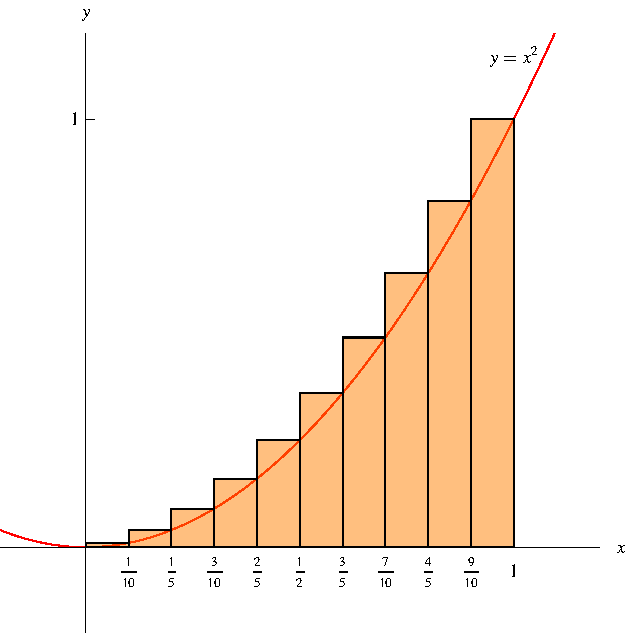
\includegraphics[height=4.2cm]{integration/pictures/05-01-righte.pdf}%
%}%
%\only<handout:0| 6>{%
%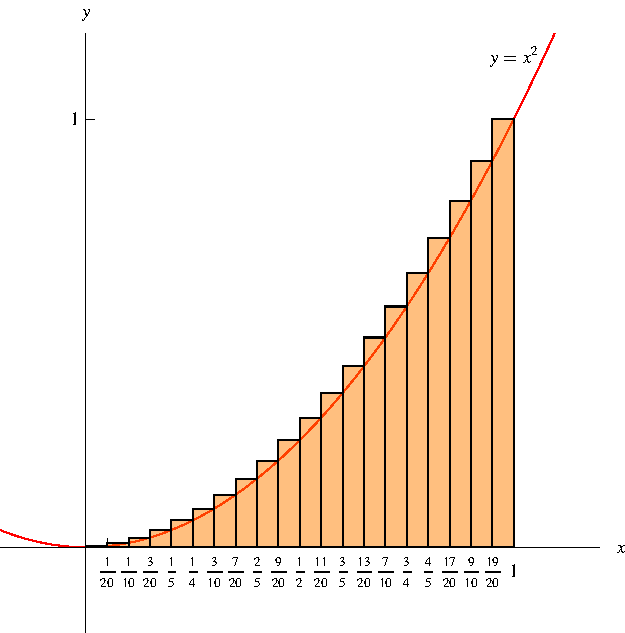
\includegraphics[height=4.2cm]{integration/pictures/05-01-rightf.pdf}%
%}%
%\only<handout:0| 7>{%
%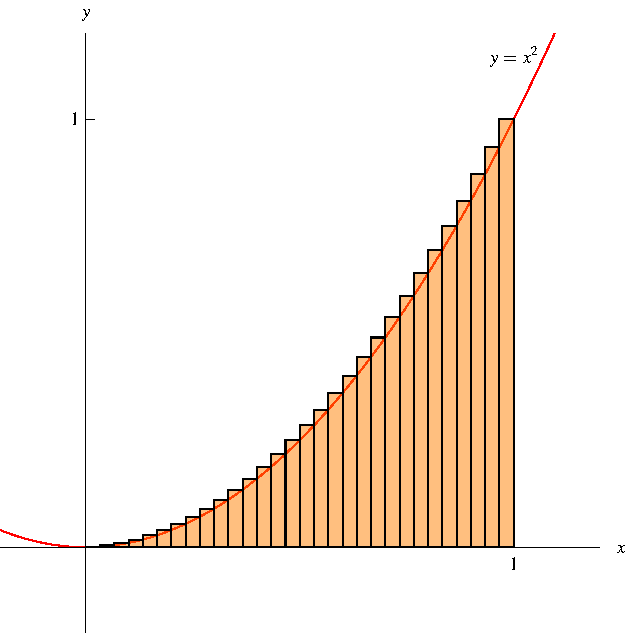
\includegraphics[height=4.2cm]{integration/pictures/05-01-rightg.pdf}%
%}%
%\only<handout:0| 8>{%
%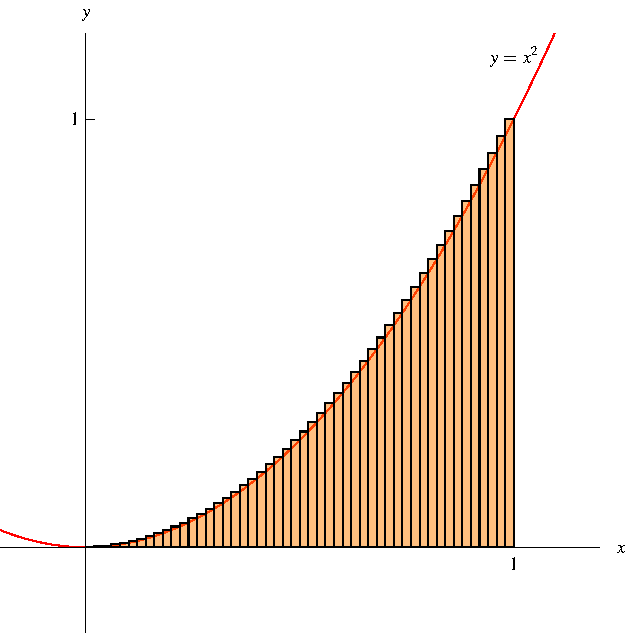
\includegraphics[height=4.2cm]{integration/pictures/05-01-righth.pdf}%
%}%
%\only<handout:1| 9->{%
%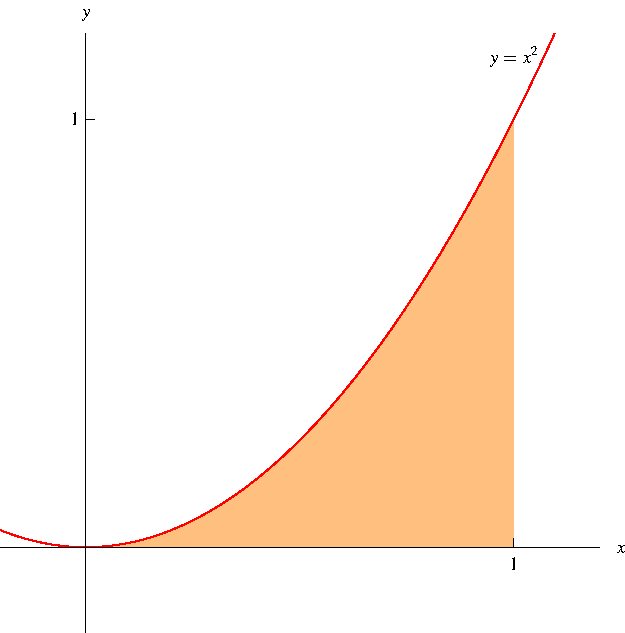
\includegraphics[height=4.2cm]{integration/pictures/05-01-xsquaredarea.pdf}%
%}%
\end{columns}
\begin{columns}
\column{.4\textwidth}


\uncover<10->{%
\psset{xunit=2cm, yunit=2cm}
\begin{pspicture}(-5, -5)(5,5) 
\psframe*[linecolor=white](-5,-5)(5,5) 
\psaxes[ticks=none, labels=none]{<->}(0,0)(-0.1,-1.2)(2,1)\tiny
\rput (1, 0.8){$y=f(x)$}

\uncover<11>{
\psline*[linecolor=\psColorNegativeAreaUnderGraph, linewidth=0.1pt](0.45, 0)(0.45, -0.582187)(0.1, -0.582187)(0.1, 0)
\psline*[linecolor=\psColorAreaUnderGraph, linewidth=0.1pt](0.8, 0)(0.8, 0.512)(0.45, 0.512)(0.45, 0)(1.15, 0)(1.15, 0.142313)(0.8, 0.142313)(0.8, 0)
\psline*[linecolor=\psColorNegativeAreaUnderGraph, linewidth=0.1pt](1.5, 0)(1.5, -0.405)(1.15, -0.405)(1.15, 0)
\psline[linecolor=brown, linewidth=0.1pt](0.45, 0)(0.45, -0.582187)(0.1, -0.582187)(0.1, 0)
\psline[linecolor=blue, linewidth=0.1pt](0.8, 0)(0.8, 0.512)(0.45, 0.512)(0.45, 0)(1.15, 0)(1.15, 0.142313)(0.8, 0.142313)(0.8, 0)
\psline[linecolor=brown, linewidth=0.1pt](1.5, 0)(1.5, -0.405)(1.15, -0.405)(1.15, 0)
}
\uncover<12>{
\psline*[linecolor=\psColorNegativeAreaUnderGraph, linewidth=0.1pt](0.333333, 0)(0.333333, -0.975802)(0.1, -0.975802)(0.1, 0)(0.566667, 0)(0.566667, -0.123617)(0.333333, -0.123617)(0.333333, 0)
\psline*[linecolor=\psColorAreaUnderGraph, linewidth=0.1pt](0.8, 0)(0.8, 0.512)(0.566667, 0.512)(0.566667, 0)(1.03333, 0)(1.03333, 0.422901)(0.8, 0.422901)(0.8, 0)
\psline*[linecolor=\psColorNegativeAreaUnderGraph, linewidth=0.1pt](1.26667, 0)(1.26667, -0.187654)(1.03333, -0.187654)(1.03333, 0)(1.5, 0)(1.5, -0.405)(1.26667, -0.405)(1.26667, 0)
\psline[linecolor=brown, linewidth=0.1pt](0.333333, 0)(0.333333, -0.975802)(0.1, -0.975802)(0.1, 0)(0.566667, 0)(0.566667, -0.123617)(0.333333, -0.123617)(0.333333, 0)
\psline[linecolor=blue, linewidth=0.1pt](0.8, 0)(0.8, 0.512)(0.566667, 0.512)(0.566667, 0)(1.03333, 0)(1.03333, 0.422901)(0.8, 0.422901)(0.8, 0)
\psline[linecolor=brown, linewidth=0.1pt](1.26667, 0)(1.26667, -0.187654)(1.03333, -0.187654)(1.03333, 0)(1.5, 0)(1.5, -0.405)(1.26667, -0.405)(1.26667, 0)
}
\uncover<13>{
\psline*[linecolor=\psColorNegativeAreaUnderGraph, linewidth=0.1pt](0.275, 0)(0.275, -1.0954)(0.1, -1.0954)(0.1, 0)(0.45, 0)(0.45, -0.582187)(0.275, -0.582187)(0.275, 0)
\psline*[linecolor=\psColorAreaUnderGraph, linewidth=0.1pt](0.625, 0)(0.625, 0.0875977)(0.45, 0.0875977)(0.45, 0)(0.8, 0)(0.8, 0.512)(0.625, 0.512)(0.625, 0)(0.975, 0)(0.975, 0.51416)(0.8, 0.51416)(0.8, 0)(1.15, 0)(1.15, 0.142313)(0.975, 0.142313)(0.975, 0)
\psline*[linecolor=\psColorNegativeAreaUnderGraph, linewidth=0.1pt](1.325, 0)(1.325, -0.330215)(1.15, -0.330215)(1.15, 0)(1.5, 0)(1.5, -0.405)(1.325, -0.405)(1.325, 0)
\psline[linecolor=brown, linewidth=0.1pt](0.275, 0)(0.275, -1.0954)(0.1, -1.0954)(0.1, 0)(0.45, 0)(0.45, -0.582187)(0.275, -0.582187)(0.275, 0)
\psline[linecolor=blue, linewidth=0.1pt](0.625, 0)(0.625, 0.0875977)(0.45, 0.0875977)(0.45, 0)(0.8, 0)(0.8, 0.512)(0.625, 0.512)(0.625, 0)(0.975, 0)(0.975, 0.51416)(0.8, 0.51416)(0.8, 0)(1.15, 0)(1.15, 0.142313)(0.975, 0.142313)(0.975, 0)
\psline[linecolor=brown, linewidth=0.1pt](1.325, 0)(1.325, -0.330215)(1.15, -0.330215)(1.15, 0)(1.5, 0)(1.5, -0.405)(1.325, -0.405)(1.325, 0)
}
\uncover<14>{
\psline*[linecolor=\psColorNegativeAreaUnderGraph, linewidth=0.1pt](0.24, 0)(0.24, -1.12804)(0.1, -1.12804)(0.1, 0)(0.38, 0)(0.38, -0.836334)(0.24, -0.836334)(0.24, 0)(0.52, 0)(0.52, -0.30551)(0.38, -0.30551)(0.38, 0)
\psline*[linecolor=\psColorAreaUnderGraph, linewidth=0.1pt](0.66, 0)(0.66, 0.20101)(0.52, 0.20101)(0.52, 0)(0.8, 0)(0.8, 0.512)(0.66, 0.512)(0.66, 0)(0.94, 0)(0.94, 0.548434)(0.8, 0.548434)(0.8, 0)(1.08, 0)(1.08, 0.323482)(0.94, 0.323482)(0.94, 0)
\psline*[linecolor=\psColorNegativeAreaUnderGraph, linewidth=0.1pt](1.22, 0)(1.22, -0.0574864)(1.08, -0.0574864)(1.08, 0)(1.36, 0)(1.36, -0.396902)(1.22, -0.396902)(1.22, 0)(1.5, 0)(1.5, -0.405)(1.36, -0.405)(1.36, 0)
\psline[linecolor=brown, linewidth=0.1pt](0.24, 0)(0.24, -1.12804)(0.1, -1.12804)(0.1, 0)(0.38, 0)(0.38, -0.836334)(0.24, -0.836334)(0.24, 0)(0.52, 0)(0.52, -0.30551)(0.38, -0.30551)(0.38, 0)
\psline[linecolor=blue, linewidth=0.1pt](0.66, 0)(0.66, 0.20101)(0.52, 0.20101)(0.52, 0)(0.8, 0)(0.8, 0.512)(0.66, 0.512)(0.66, 0)(0.94, 0)(0.94, 0.548434)(0.8, 0.548434)(0.8, 0)(1.08, 0)(1.08, 0.323482)(0.94, 0.323482)(0.94, 0)
\psline[linecolor=brown, linewidth=0.1pt](1.22, 0)(1.22, -0.0574864)(1.08, -0.0574864)(1.08, 0)(1.36, 0)(1.36, -0.396902)(1.22, -0.396902)(1.22, 0)(1.5, 0)(1.5, -0.405)(1.36, -0.405)(1.36, 0)
}
\uncover<15>{
\psline*[linecolor=\psColorNegativeAreaUnderGraph, linewidth=0.1pt](0.193333, 0)(0.193333, -1.11333)(0.1, -1.11333)(0.1, 0)(0.286667, 0)(0.286667, -1.07743)(0.193333, -1.07743)(0.193333, 0)(0.38, 0)(0.38, -0.836334)(0.286667, -0.836334)(0.286667, 0)(0.473333, 0)(0.473333, -0.490863)(0.38, -0.490863)(0.38, 0)(0.566667, 0)(0.566667, -0.123617)(0.473333, -0.123617)(0.473333, 0)
\psline*[linecolor=\psColorAreaUnderGraph, linewidth=0.1pt](0.66, 0)(0.66, 0.20101)(0.566667, 0.20101)(0.566667, 0)(0.753333, 0)(0.753333, 0.436837)(0.66, 0.436837)(0.66, 0)(0.846667, 0)(0.846667, 0.555898)(0.753333, 0.555898)(0.753333, 0)(0.94, 0)(0.94, 0.548434)(0.846667, 0.548434)(0.846667, 0)(1.03333, 0)(1.03333, 0.422901)(0.94, 0.422901)(0.94, 0)(1.12667, 0)(1.12667, 0.205968)(1.03333, 0.205968)(1.03333, 0)
\psline*[linecolor=\psColorNegativeAreaUnderGraph, linewidth=0.1pt](1.22, 0)(1.22, -0.0574864)(1.12667, -0.0574864)(1.12667, 0)(1.31333, 0)(1.31333, -0.30437)(1.22, -0.30437)(1.22, 0)(1.40667, 0)(1.40667, -0.45338)(1.31333, -0.45338)(1.31333, 0)(1.5, 0)(1.5, -0.405)(1.40667, -0.405)(1.40667, 0)
\psline[linecolor=brown, linewidth=0.1pt](0.193333, 0)(0.193333, -1.11333)(0.1, -1.11333)(0.1, 0)(0.286667, 0)(0.286667, -1.07743)(0.193333, -1.07743)(0.193333, 0)(0.38, 0)(0.38, -0.836334)(0.286667, -0.836334)(0.286667, 0)(0.473333, 0)(0.473333, -0.490863)(0.38, -0.490863)(0.38, 0)(0.566667, 0)(0.566667, -0.123617)(0.473333, -0.123617)(0.473333, 0)
\psline[linecolor=blue, linewidth=0.1pt](0.66, 0)(0.66, 0.20101)(0.566667, 0.20101)(0.566667, 0)(0.753333, 0)(0.753333, 0.436837)(0.66, 0.436837)(0.66, 0)(0.846667, 0)(0.846667, 0.555898)(0.753333, 0.555898)(0.753333, 0)(0.94, 0)(0.94, 0.548434)(0.846667, 0.548434)(0.846667, 0)(1.03333, 0)(1.03333, 0.422901)(0.94, 0.422901)(0.94, 0)(1.12667, 0)(1.12667, 0.205968)(1.03333, 0.205968)(1.03333, 0)
\psline[linecolor=brown, linewidth=0.1pt](1.22, 0)(1.22, -0.0574864)(1.12667, -0.0574864)(1.12667, 0)(1.31333, 0)(1.31333, -0.30437)(1.22, -0.30437)(1.22, 0)(1.40667, 0)(1.40667, -0.45338)(1.31333, -0.45338)(1.31333, 0)(1.5, 0)(1.5, -0.405)(1.40667, -0.405)(1.40667, 0)
}
\uncover<16>{
\psline*[linecolor=\psColorNegativeAreaUnderGraph, linewidth=0.1pt](0.17, 0)(0.17, -1.07669)(0.1, -1.07669)(0.1, 0)(0.24, 0)(0.24, -1.12804)(0.17, -1.12804)(0.17, 0)(0.31, 0)(0.31, -1.03214)(0.24, -1.03214)(0.24, 0)(0.38, 0)(0.38, -0.836334)(0.31, -0.836334)(0.31, 0)(0.45, 0)(0.45, -0.582187)(0.38, -0.582187)(0.38, 0)(0.52, 0)(0.52, -0.30551)(0.45, -0.30551)(0.45, 0)(0.59, 0)(0.59, -0.0363499)(0.52, -0.0363499)(0.52, 0)
\psline*[linecolor=\psColorAreaUnderGraph, linewidth=0.1pt](0.66, 0)(0.66, 0.20101)(0.59, 0.20101)(0.59, 0)(0.73, 0)(0.73, 0.388046)(0.66, 0.388046)(0.66, 0)(0.8, 0)(0.8, 0.512)(0.73, 0.512)(0.73, 0)(0.87, 0)(0.87, 0.565874)(0.8, 0.565874)(0.8, 0)(0.94, 0)(0.94, 0.548434)(0.87, 0.548434)(0.87, 0)(1.01, 0)(1.01, 0.464206)(0.94, 0.464206)(0.94, 0)(1.08, 0)(1.08, 0.323482)(1.01, 0.323482)(1.01, 0)(1.15, 0)(1.15, 0.142313)(1.08, 0.142313)(1.08, 0)
\psline*[linecolor=\psColorNegativeAreaUnderGraph, linewidth=0.1pt](1.22, 0)(1.22, -0.0574864)(1.15, -0.0574864)(1.15, 0)(1.29, 0)(1.29, -0.248338)(1.22, -0.248338)(1.22, 0)(1.36, 0)(1.36, -0.396902)(1.29, -0.396902)(1.29, 0)(1.43, 0)(1.43, -0.464078)(1.36, -0.464078)(1.36, 0)(1.5, 0)(1.5, -0.405)(1.43, -0.405)(1.43, 0)
\psline[linecolor=brown, linewidth=0.1pt](0.17, 0)(0.17, -1.07669)(0.1, -1.07669)(0.1, 0)(0.24, 0)(0.24, -1.12804)(0.17, -1.12804)(0.17, 0)(0.31, 0)(0.31, -1.03214)(0.24, -1.03214)(0.24, 0)(0.38, 0)(0.38, -0.836334)(0.31, -0.836334)(0.31, 0)(0.45, 0)(0.45, -0.582187)(0.38, -0.582187)(0.38, 0)(0.52, 0)(0.52, -0.30551)(0.45, -0.30551)(0.45, 0)(0.59, 0)(0.59, -0.0363499)(0.52, -0.0363499)(0.52, 0)
\psline[linecolor=blue, linewidth=0.1pt](0.66, 0)(0.66, 0.20101)(0.59, 0.20101)(0.59, 0)(0.73, 0)(0.73, 0.388046)(0.66, 0.388046)(0.66, 0)(0.8, 0)(0.8, 0.512)(0.73, 0.512)(0.73, 0)(0.87, 0)(0.87, 0.565874)(0.8, 0.565874)(0.8, 0)(0.94, 0)(0.94, 0.548434)(0.87, 0.548434)(0.87, 0)(1.01, 0)(1.01, 0.464206)(0.94, 0.464206)(0.94, 0)(1.08, 0)(1.08, 0.323482)(1.01, 0.323482)(1.01, 0)(1.15, 0)(1.15, 0.142313)(1.08, 0.142313)(1.08, 0)
\psline[linecolor=brown, linewidth=0.1pt](1.22, 0)(1.22, -0.0574864)(1.15, -0.0574864)(1.15, 0)(1.29, 0)(1.29, -0.248338)(1.22, -0.248338)(1.22, 0)(1.36, 0)(1.36, -0.396902)(1.29, -0.396902)(1.29, 0)(1.43, 0)(1.43, -0.464078)(1.36, -0.464078)(1.36, 0)(1.5, 0)(1.5, -0.405)(1.43, -0.405)(1.43, 0)
}
\uncover<17>{
\psline*[linecolor=\psColorNegativeAreaUnderGraph, linewidth=0.1pt](0.146667, 0)(0.146667, -1.01784)(0.1, -1.01784)(0.1, 0)(0.193333, 0)(0.193333, -1.11333)(0.146667, -1.11333)(0.146667, 0)(0.24, 0)(0.24, -1.12804)(0.193333, -1.12804)(0.193333, 0)(0.286667, 0)(0.286667, -1.07743)(0.24, -1.07743)(0.24, 0)(0.333333, 0)(0.333333, -0.975802)(0.286667, -0.975802)(0.286667, 0)(0.38, 0)(0.38, -0.836334)(0.333333, -0.836334)(0.333333, 0)(0.426667, 0)(0.426667, -0.671056)(0.38, -0.671056)(0.38, 0)(0.473333, 0)(0.473333, -0.490863)(0.426667, -0.490863)(0.426667, 0)(0.52, 0)(0.52, -0.30551)(0.473333, -0.30551)(0.473333, 0)(0.566667, 0)(0.566667, -0.123617)(0.52, -0.123617)(0.52, 0)
\psline*[linecolor=\psColorAreaUnderGraph, linewidth=0.1pt](0.613333, 0)(0.613333, 0.0473366)(0.566667, 0.0473366)(0.566667, 0)(0.66, 0)(0.66, 0.20101)(0.613333, 0.20101)(0.613333, 0)(0.706667, 0)(0.706667, 0.332198)(0.66, 0.332198)(0.66, 0)(0.753333, 0)(0.753333, 0.436837)(0.706667, 0.436837)(0.706667, 0)(0.8, 0)(0.8, 0.512)(0.753333, 0.512)(0.753333, 0)(0.846667, 0)(0.846667, 0.555898)(0.8, 0.555898)(0.8, 0)(0.893333, 0)(0.893333, 0.567879)(0.846667, 0.567879)(0.846667, 0)(0.94, 0)(0.94, 0.548434)(0.893333, 0.548434)(0.893333, 0)(0.986667, 0)(0.986667, 0.499186)(0.94, 0.499186)(0.94, 0)(1.03333, 0)(1.03333, 0.422901)(0.986667, 0.422901)(0.986667, 0)(1.08, 0)(1.08, 0.323482)(1.03333, 0.323482)(1.03333, 0)(1.12667, 0)(1.12667, 0.205968)(1.08, 0.205968)(1.08, 0)(1.17333, 0)(1.17333, 0.0765396)(1.12667, 0.0765396)(1.12667, 0)
\psline*[linecolor=\psColorNegativeAreaUnderGraph, linewidth=0.1pt](1.22, 0)(1.22, -0.0574864)(1.17333, -0.0574864)(1.17333, 0)(1.26667, 0)(1.26667, -0.187654)(1.22, -0.187654)(1.22, 0)(1.31333, 0)(1.31333, -0.30437)(1.26667, -0.30437)(1.26667, 0)(1.36, 0)(1.36, -0.396902)(1.31333, -0.396902)(1.31333, 0)(1.40667, 0)(1.40667, -0.45338)(1.36, -0.45338)(1.36, 0)(1.45333, 0)(1.45333, -0.460795)(1.40667, -0.460795)(1.40667, 0)(1.5, 0)(1.5, -0.405)(1.45333, -0.405)(1.45333, 0)
\psline[linecolor=brown, linewidth=0.1pt](0.146667, 0)(0.146667, -1.01784)(0.1, -1.01784)(0.1, 0)(0.193333, 0)(0.193333, -1.11333)(0.146667, -1.11333)(0.146667, 0)(0.24, 0)(0.24, -1.12804)(0.193333, -1.12804)(0.193333, 0)(0.286667, 0)(0.286667, -1.07743)(0.24, -1.07743)(0.24, 0)(0.333333, 0)(0.333333, -0.975802)(0.286667, -0.975802)(0.286667, 0)(0.38, 0)(0.38, -0.836334)(0.333333, -0.836334)(0.333333, 0)(0.426667, 0)(0.426667, -0.671056)(0.38, -0.671056)(0.38, 0)(0.473333, 0)(0.473333, -0.490863)(0.426667, -0.490863)(0.426667, 0)(0.52, 0)(0.52, -0.30551)(0.473333, -0.30551)(0.473333, 0)(0.566667, 0)(0.566667, -0.123617)(0.52, -0.123617)(0.52, 0)
\psline[linecolor=blue, linewidth=0.1pt](0.613333, 0)(0.613333, 0.0473366)(0.566667, 0.0473366)(0.566667, 0)(0.66, 0)(0.66, 0.20101)(0.613333, 0.20101)(0.613333, 0)(0.706667, 0)(0.706667, 0.332198)(0.66, 0.332198)(0.66, 0)(0.753333, 0)(0.753333, 0.436837)(0.706667, 0.436837)(0.706667, 0)(0.8, 0)(0.8, 0.512)(0.753333, 0.512)(0.753333, 0)(0.846667, 0)(0.846667, 0.555898)(0.8, 0.555898)(0.8, 0)(0.893333, 0)(0.893333, 0.567879)(0.846667, 0.567879)(0.846667, 0)(0.94, 0)(0.94, 0.548434)(0.893333, 0.548434)(0.893333, 0)(0.986667, 0)(0.986667, 0.499186)(0.94, 0.499186)(0.94, 0)(1.03333, 0)(1.03333, 0.422901)(0.986667, 0.422901)(0.986667, 0)(1.08, 0)(1.08, 0.323482)(1.03333, 0.323482)(1.03333, 0)(1.12667, 0)(1.12667, 0.205968)(1.08, 0.205968)(1.08, 0)(1.17333, 0)(1.17333, 0.0765396)(1.12667, 0.0765396)(1.12667, 0)
\psline[linecolor=brown, linewidth=0.1pt](1.22, 0)(1.22, -0.0574864)(1.17333, -0.0574864)(1.17333, 0)(1.26667, 0)(1.26667, -0.187654)(1.22, -0.187654)(1.22, 0)(1.31333, 0)(1.31333, -0.30437)(1.26667, -0.30437)(1.26667, 0)(1.36, 0)(1.36, -0.396902)(1.31333, -0.396902)(1.31333, 0)(1.40667, 0)(1.40667, -0.45338)(1.36, -0.45338)(1.36, 0)(1.45333, 0)(1.45333, -0.460795)(1.40667, -0.460795)(1.40667, 0)(1.5, 0)(1.5, -0.405)(1.45333, -0.405)(1.45333, 0)
}
\uncover<18>{
\psline*[linecolor=\psColorNegativeAreaUnderGraph, linewidth=0.1pt](0.135, 0)(0.135, -0.979431)(0.1, -0.979431)(0.1, 0)(0.17, 0)(0.17, -1.07669)(0.135, -1.07669)(0.135, 0)(0.205, 0)(0.205, -1.12395)(0.17, -1.12395)(0.17, 0)(0.24, 0)(0.24, -1.12804)(0.205, -1.12804)(0.205, 0)(0.275, 0)(0.275, -1.0954)(0.24, -1.0954)(0.24, 0)(0.31, 0)(0.31, -1.03214)(0.275, -1.03214)(0.275, 0)(0.345, 0)(0.345, -0.943994)(0.31, -0.943994)(0.31, 0)(0.38, 0)(0.38, -0.836334)(0.345, -0.836334)(0.345, 0)(0.415, 0)(0.415, -0.71418)(0.38, -0.71418)(0.38, 0)(0.45, 0)(0.45, -0.582187)(0.415, -0.582187)(0.415, 0)(0.485, 0)(0.485, -0.444652)(0.45, -0.444652)(0.45, 0)(0.52, 0)(0.52, -0.30551)(0.485, -0.30551)(0.485, 0)(0.555, 0)(0.555, -0.168338)(0.52, -0.168338)(0.52, 0)(0.59, 0)(0.59, -0.0363499)(0.555, -0.0363499)(0.555, 0)
\psline*[linecolor=\psColorAreaUnderGraph, linewidth=0.1pt](0.625, 0)(0.625, 0.0875977)(0.59, 0.0875977)(0.59, 0)(0.66, 0)(0.66, 0.20101)(0.625, 0.20101)(0.625, 0)(0.695, 0)(0.695, 0.301751)(0.66, 0.301751)(0.66, 0)(0.73, 0)(0.73, 0.388046)(0.695, 0.388046)(0.695, 0)(0.765, 0)(0.765, 0.458481)(0.73, 0.458481)(0.73, 0)(0.8, 0)(0.8, 0.512)(0.765, 0.512)(0.765, 0)(0.835, 0)(0.835, 0.547909)(0.8, 0.547909)(0.8, 0)(0.87, 0)(0.87, 0.565874)(0.835, 0.565874)(0.835, 0)(0.905, 0)(0.905, 0.56592)(0.87, 0.56592)(0.87, 0)(0.94, 0)(0.94, 0.548434)(0.905, 0.548434)(0.905, 0)(0.975, 0)(0.975, 0.51416)(0.94, 0.51416)(0.94, 0)(1.01, 0)(1.01, 0.464206)(0.975, 0.464206)(0.975, 0)(1.045, 0)(1.045, 0.400038)(1.01, 0.400038)(1.01, 0)(1.08, 0)(1.08, 0.323482)(1.045, 0.323482)(1.045, 0)(1.115, 0)(1.115, 0.236724)(1.08, 0.236724)(1.08, 0)(1.15, 0)(1.15, 0.142313)(1.115, 0.142313)(1.115, 0)(1.185, 0)(1.185, 0.0431533)(1.15, 0.0431533)(1.15, 0)
\psline*[linecolor=\psColorNegativeAreaUnderGraph, linewidth=0.1pt](1.22, 0)(1.22, -0.0574864)(1.185, -0.0574864)(1.185, 0)(1.255, 0)(1.255, -0.155979)(1.22, -0.155979)(1.22, 0)(1.29, 0)(1.29, -0.248338)(1.255, -0.248338)(1.255, 0)(1.325, 0)(1.325, -0.330215)(1.29, -0.330215)(1.29, 0)(1.36, 0)(1.36, -0.396902)(1.325, -0.396902)(1.325, 0)(1.395, 0)(1.395, -0.443333)(1.36, -0.443333)(1.36, 0)(1.43, 0)(1.43, -0.464078)(1.395, -0.464078)(1.395, 0)(1.465, 0)(1.465, -0.45335)(1.43, -0.45335)(1.43, 0)(1.5, 0)(1.5, -0.405)(1.465, -0.405)(1.465, 0)
\psline[linecolor=brown, linewidth=0.1pt](0.135, 0)(0.135, -0.979431)(0.1, -0.979431)(0.1, 0)(0.17, 0)(0.17, -1.07669)(0.135, -1.07669)(0.135, 0)(0.205, 0)(0.205, -1.12395)(0.17, -1.12395)(0.17, 0)(0.24, 0)(0.24, -1.12804)(0.205, -1.12804)(0.205, 0)(0.275, 0)(0.275, -1.0954)(0.24, -1.0954)(0.24, 0)(0.31, 0)(0.31, -1.03214)(0.275, -1.03214)(0.275, 0)(0.345, 0)(0.345, -0.943994)(0.31, -0.943994)(0.31, 0)(0.38, 0)(0.38, -0.836334)(0.345, -0.836334)(0.345, 0)(0.415, 0)(0.415, -0.71418)(0.38, -0.71418)(0.38, 0)(0.45, 0)(0.45, -0.582187)(0.415, -0.582187)(0.415, 0)(0.485, 0)(0.485, -0.444652)(0.45, -0.444652)(0.45, 0)(0.52, 0)(0.52, -0.30551)(0.485, -0.30551)(0.485, 0)(0.555, 0)(0.555, -0.168338)(0.52, -0.168338)(0.52, 0)(0.59, 0)(0.59, -0.0363499)(0.555, -0.0363499)(0.555, 0)
\psline[linecolor=blue, linewidth=0.1pt](0.625, 0)(0.625, 0.0875977)(0.59, 0.0875977)(0.59, 0)(0.66, 0)(0.66, 0.20101)(0.625, 0.20101)(0.625, 0)(0.695, 0)(0.695, 0.301751)(0.66, 0.301751)(0.66, 0)(0.73, 0)(0.73, 0.388046)(0.695, 0.388046)(0.695, 0)(0.765, 0)(0.765, 0.458481)(0.73, 0.458481)(0.73, 0)(0.8, 0)(0.8, 0.512)(0.765, 0.512)(0.765, 0)(0.835, 0)(0.835, 0.547909)(0.8, 0.547909)(0.8, 0)(0.87, 0)(0.87, 0.565874)(0.835, 0.565874)(0.835, 0)(0.905, 0)(0.905, 0.56592)(0.87, 0.56592)(0.87, 0)(0.94, 0)(0.94, 0.548434)(0.905, 0.548434)(0.905, 0)(0.975, 0)(0.975, 0.51416)(0.94, 0.51416)(0.94, 0)(1.01, 0)(1.01, 0.464206)(0.975, 0.464206)(0.975, 0)(1.045, 0)(1.045, 0.400038)(1.01, 0.400038)(1.01, 0)(1.08, 0)(1.08, 0.323482)(1.045, 0.323482)(1.045, 0)(1.115, 0)(1.115, 0.236724)(1.08, 0.236724)(1.08, 0)(1.15, 0)(1.15, 0.142313)(1.115, 0.142313)(1.115, 0)(1.185, 0)(1.185, 0.0431533)(1.15, 0.0431533)(1.15, 0)
\psline[linecolor=brown, linewidth=0.1pt](1.22, 0)(1.22, -0.0574864)(1.185, -0.0574864)(1.185, 0)(1.255, 0)(1.255, -0.155979)(1.22, -0.155979)(1.22, 0)(1.29, 0)(1.29, -0.248338)(1.255, -0.248338)(1.255, 0)(1.325, 0)(1.325, -0.330215)(1.29, -0.330215)(1.29, 0)(1.36, 0)(1.36, -0.396902)(1.325, -0.396902)(1.325, 0)(1.395, 0)(1.395, -0.443333)(1.36, -0.443333)(1.36, 0)(1.43, 0)(1.43, -0.464078)(1.395, -0.464078)(1.395, 0)(1.465, 0)(1.465, -0.45335)(1.43, -0.45335)(1.43, 0)(1.5, 0)(1.5, -0.405)(1.465, -0.405)(1.465, 0)
}

\uncover<19->{
\pscustom*[linecolor=\psColorNegativeAreaUnderGraph]{
\psplot{0.1}{0.6}{x 3 exp -34 mul x -11.52 mul x 4 exp 10 mul x 2 exp 36 mul add add add }
\psline(0.6,0)(0.1,0)
}
\pscustom*[linecolor=\psColorAreaUnderGraph]{
\psplot{0.6}{1.2}{x 3 exp -34 mul x -11.52 mul x 4 exp 10 mul x 2 exp 36 mul add add add }
\psline(1.2,0)(0.6,0)
}
\pscustom*[linecolor=\psColorNegativeAreaUnderGraph]{
\psplot{1.2}{1.5}{x 3 exp -34 mul x -11.52 mul x 4 exp 10 mul x 2 exp 36 mul add add add }
\psline(1.5,0)(1.2,0)
}
}
\psplot[linecolor=red, plotpoints=1000]{0.1}{1.5}{x 3 exp -34 mul x -11.52 mul x 4 exp 10 mul x 2 exp 36 mul add add add }
\uncover<19->{
\rput (0.9, 0.3){$A_1$}
\rput[t](0.9, -0.5){$A_2$}
\psline{->}(0.85, -0.45)(0.35, -0.3)
\psline{->}(0.95, -0.45)(1.4, -0.2)
}
\end{pspicture} 
%\only<handout:0| -10>{%
%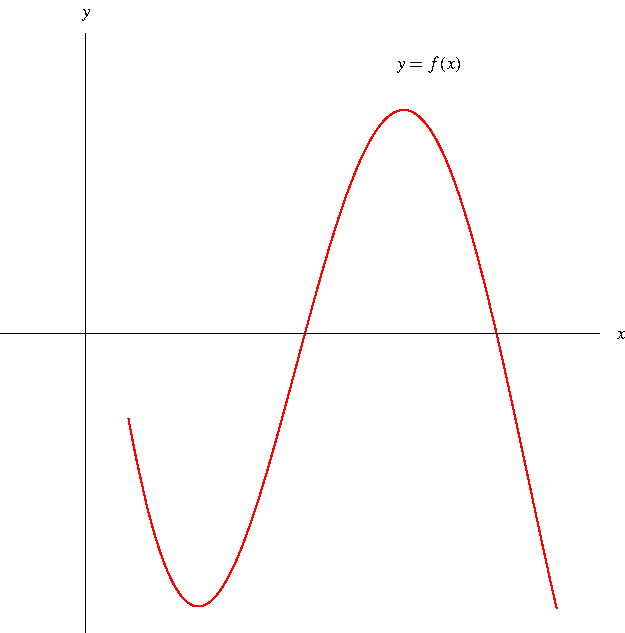
\includegraphics[height=4.2cm]{integration/pictures/05-02-net-area-function.pdf}%
%}%
%\only<handout:0| 11>{%
%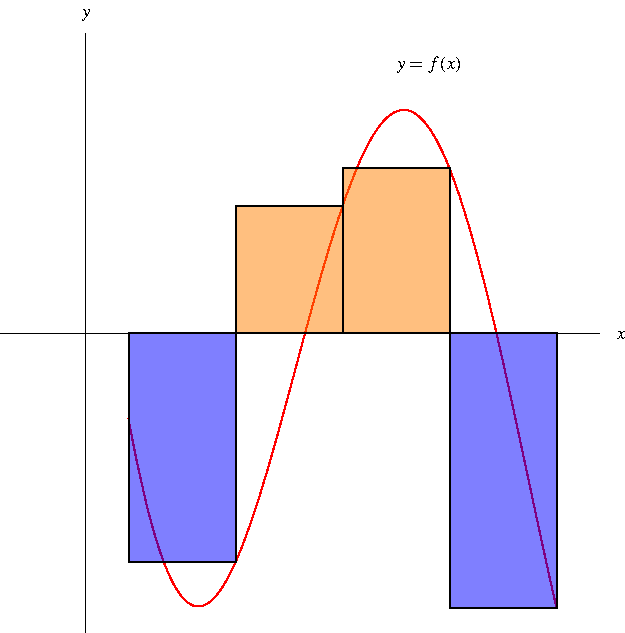
\includegraphics[height=4.2cm]{integration/pictures/05-02-net-areaa.pdf}%
%}%
%\only<handout:0| 12>{%
%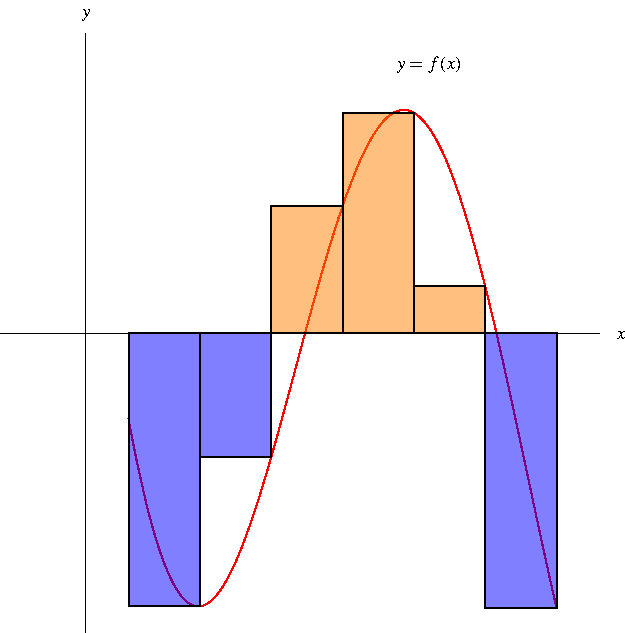
\includegraphics[height=4.2cm]{integration/pictures/05-02-net-areab.pdf}%
%}%
%\only<handout:0| 13>{%
%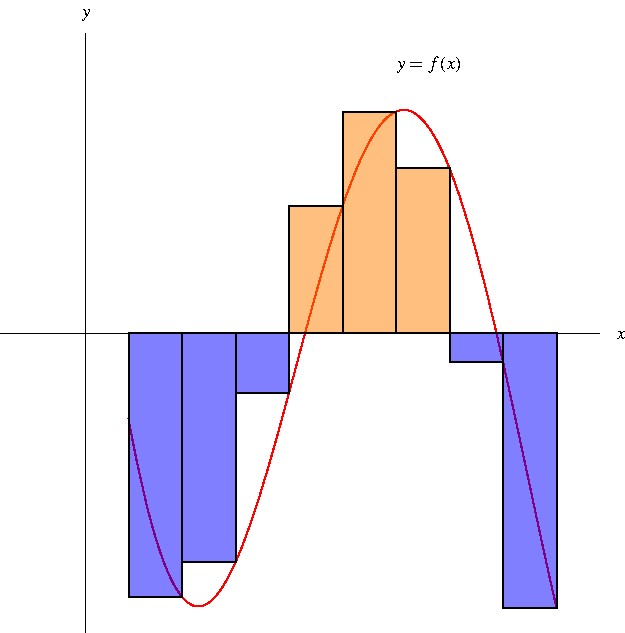
\includegraphics[height=4.2cm]{integration/pictures/05-02-net-areac.pdf}%
%}%
%\only<handout:0| 14>{%
%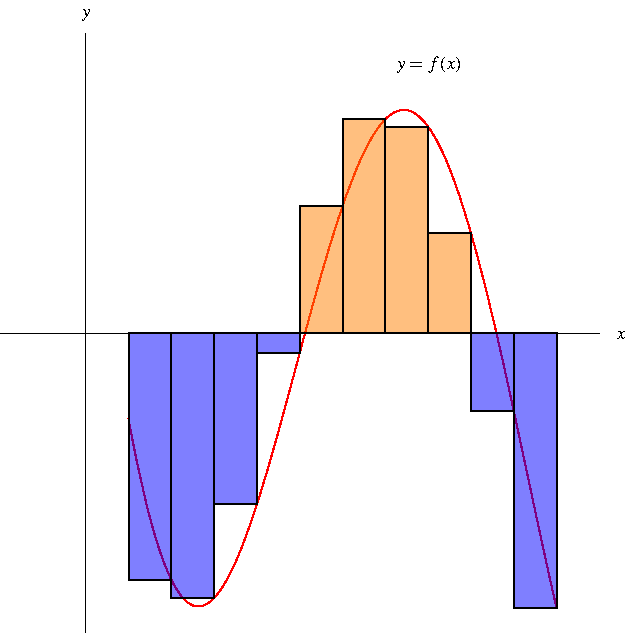
\includegraphics[height=4.2cm]{integration/pictures/05-02-net-aread.pdf}%
%}%
%\only<handout:0| 15>{%
%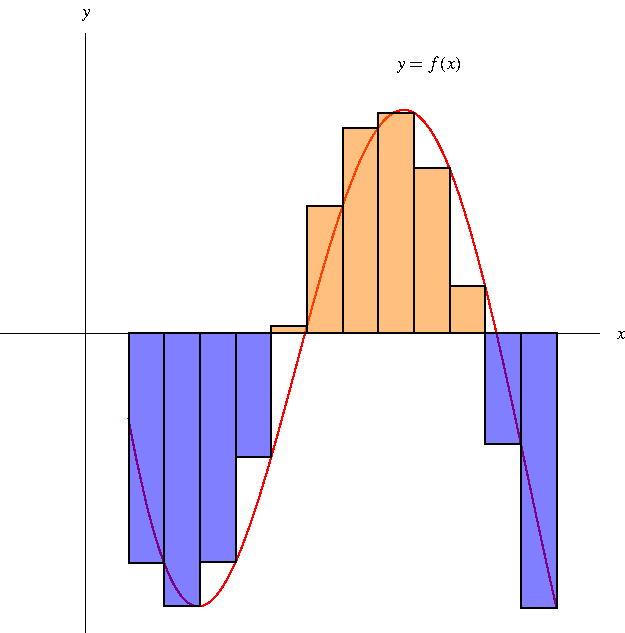
\includegraphics[height=4.2cm]{integration/pictures/05-02-net-areae.pdf}%
%}%
%\only<handout:0| 16>{%
%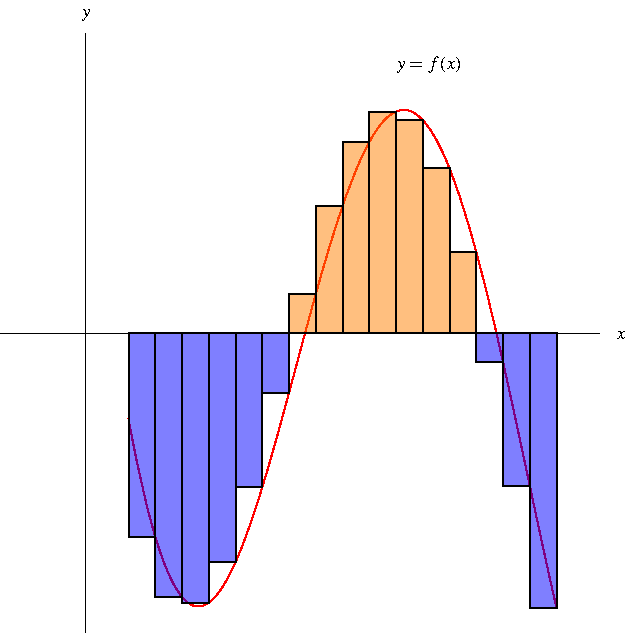
\includegraphics[height=4.2cm]{integration/pictures/05-02-net-areaf.pdf}%
%}%
%\only<handout:0| 17>{%
%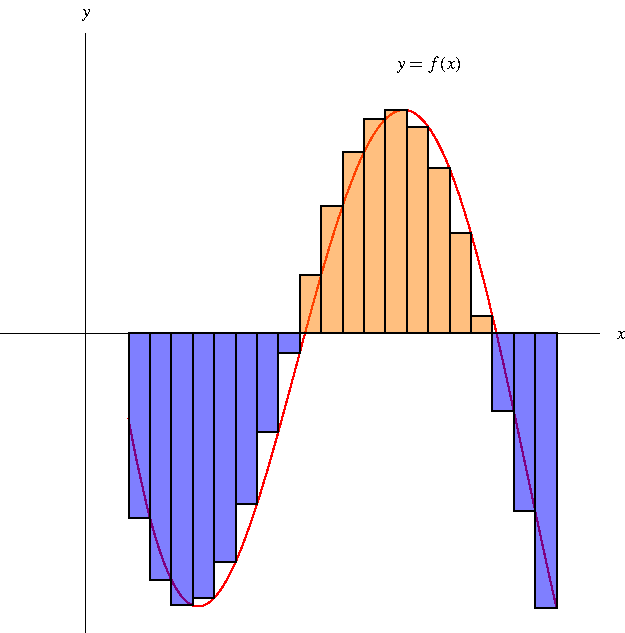
\includegraphics[height=4.2cm]{integration/pictures/05-02-net-areag.pdf}%
%}%
%\only<handout:0| 18>{%
%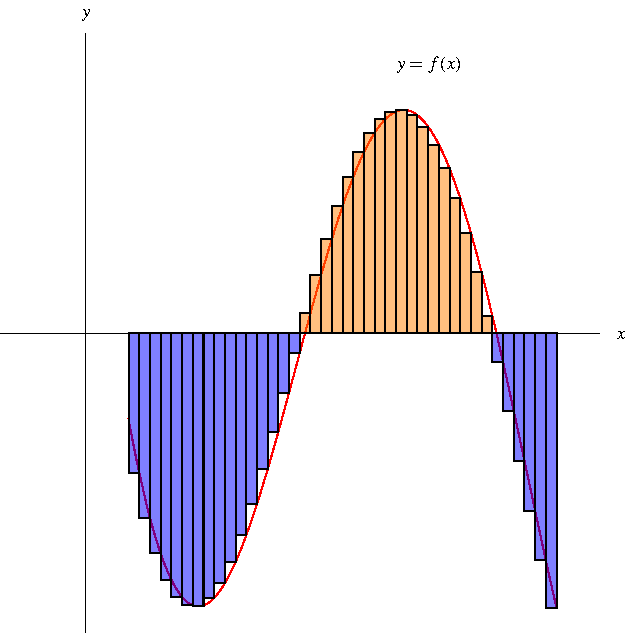
\includegraphics[height=4.2cm]{integration/pictures/05-02-net-areah.pdf}%
%}%
%\only<handout:1| 19->{%
%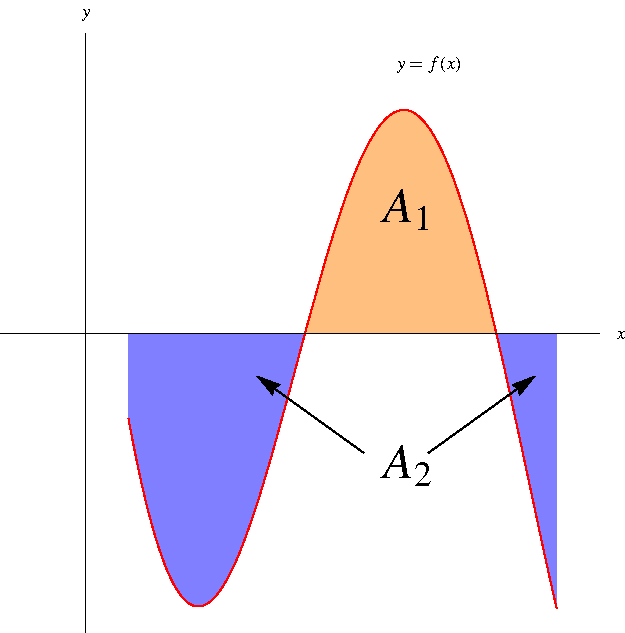
\includegraphics[height=4.2cm]{integration/pictures/05-02-net-area-limit.pdf}%
%}%
}%
\column{.6\textwidth}
\begin{itemize}
\item<10->  What if $f(x)$ is sometimes negative?
\item<19->  Then $\int_a^bf(x)\diff x = A_1 - A_2$.
\item<19->  $A_1$ is the area of the region above the $x$-axis and below the graph of $f$.
\item<19->  $A_2$ is the area of the region below the $x$-axis and above the graph of $f$.
\end{itemize}
\end{columns}
\end{frame}
% end module definite-integral-negative
